\documentclass[11pt]{article}
\usepackage[margin=1in]{geometry}
\usepackage{amsmath,amssymb,booktabs,graphicx,hyperref,xcolor,array,subcaption}
\graphicspath{{../plots/}}
\title{Learning Without Backpropagation: A Controlled Comparison of \\ Feedback Alignment, Target Propagation, Forward-Forward, Equilibrium Propagation and Weight Perturbation}
\author{Tabish Shah Mohsin \\ Zakir Husain College of Engineering and Technology, Aligarh Muslim University}
\date{\today}
\newcommand{\todo}[1]{{\color{red}[TODO: #1]}}
\begin{document}
\maketitle

\begin{abstract}
Backpropagation (BP) is the workhorse of deep learning, yet it is widely regarded as biologically implausible and awkward on neuromorphic hardware because it needs weight transport, a separate backward phase and global, non-local error signals. A large literature proposes alternatives. We review six of them---Feedback Alignment (FA), Direct Feedback Alignment (DFA), Difference Target Propagation (DTP), the Forward-Forward algorithm (FF), Equilibrium Propagation (EqProp) and weight perturbation (SPSA)---and compare them with BP in a controlled benchmark: the same 784-256-128-10 network, data split, optimizer family, learning-rate schedule and validation-based tuning protocol, with every update rule implemented by hand and without autograd. Beyond accuracy we measure convergence speed, generalisation gap, measured multiply-accumulate cost, robustness to depth and to small data, and---for each method---the cosine alignment between its update and the true gradient. On MNIST, BP reaches 98.5\%; Equilibrium Propagation comes within 0.6 points but costs $28\times$ more multiply-accumulates, FA and DFA lose about one point, DTP and Forward-Forward lose 2.5--4 points, and weight perturbation with 16 directions reaches 90.8\%. Measured gradient alignment explains part of this: hidden-layer updates of FA/DFA have cosine $\approx0.4$ with the true gradient, and the alignment of SPSA matches the theoretical $\sqrt{k/(d+k)}$ law. With depth, BP is unaffected while FA, DFA and DTP degrade markedly (6 hidden layers: 89\%, 92\%, 26\%). \todo{Fashion-MNIST numbers: run on Colab and update abstract.}
\end{abstract}

\section{Introduction}
Error backpropagation \cite{rumelhart1986} computes exact gradients by running the network's computation graph backwards. Three properties of that procedure are problematic outside a GPU: (i) the backward pass uses the transpose of the forward weights (the \emph{weight transport} problem \cite{grossberg1987,crick1989}); (ii) neurons must alternate between a forward and a backward phase and store forward activity until the error arrives; (iii) the update of a synapse depends on a signal that is computed far away in the network, so it is not \emph{local}. Reviews of these issues from the neuroscience side include \cite{whittington2019,lillicrap2020}; from the machine-learning side, \cite{bartunov2018,xiao2018,baydin2022}.

This paper does two things. First, Section~\ref{sec:methods} gives a unified description of six alternatives, expressed as the update rule each one applies to the same network. Second, Sections~\ref{sec:setup}--\ref{sec:results} report a controlled experimental comparison whose axes follow the properties above: accuracy, learning speed, computational cost, quality of the gradient estimate, scaling with depth, and data efficiency.

\paragraph{Contributions.} (1) A single code base (PyTorch, no autograd in any learning rule) in which all methods share data, architecture family, optimizer and tuning protocol. (2) A direct measurement of gradient alignment for every method that has a gradient to compare with, including EqProp against back-propagation-through-time of its own relaxation. (3) An empirical study of how alignment, accuracy and cost change with depth, data size and (for SPSA and EqProp) the estimator's hyper-parameters.

\section{Background and taxonomy}
Let a network have layers $a_l = f(z_l)$, $z_l = W_l a_{l-1} + b_l$, and loss $\mathcal{L}$. BP sets $\delta_L=\nabla_{z_L}\mathcal L$ and $\delta_l = (W_{l+1}^\top\delta_{l+1})\odot f'(z_l)$, $\Delta W_l=-\eta\,\delta_l a_{l-1}^\top$. Table~\ref{tab:taxonomy} classifies the alternatives by which of BP's requirements they remove.

\begin{table}[h]\centering\small
\begin{tabular}{lcccc}\toprule
Method & Weight transport & Separate backward pass & Update local in space & Estimator of $\nabla\mathcal L$ \\ \midrule
BP & yes & yes & no & exact \\
FA & no (fixed random $B$) & yes & partly & biased, learned alignment \\
DFA & no & no (broadcast of $e$) & partly & biased \\
DTP & no (learned inverses) & feedback network & yes, given targets & biased \\
FF & no & no & yes (layer-wise objective) & different objective \\
EqProp & symmetric weights & no (second relaxation) & yes (Hebbian) & $\to$ exact as $\beta\to0$ \\
SPSA & no & no & no (global scalar) & unbiased, high variance \\ \bottomrule
\end{tabular}
\caption{Qualitative taxonomy of the compared learning rules.}\label{tab:taxonomy}
\end{table}

\section{Methods}\label{sec:methods}
All methods below train the MLP $784\!\to\!256\!\to\!128\!\to\!10$ (except where stated) and produce, for a mini-batch, an update direction that is passed to a common optimizer.

\paragraph{Feedback Alignment \cite{lillicrap2016}.} Replace $W_{l+1}^\top$ in the backward recursion by a fixed random matrix $B_{l+1}$: $\delta_l=(B_{l+1}\delta_{l+1})\odot f'(z_l)$. The forward weights come to align with $B$ so that the resulting update correlates positively with the true gradient \cite{lillicrap2016,refinetti2021}.

\paragraph{Direct Feedback Alignment \cite{nokland2016}.} The output error $e$ is projected directly to every hidden layer, $\delta_l=(B_l e)\odot f'(z_l)$, removing the layer-to-layer backward chain \cite{launay2020}.

\paragraph{Difference Target Propagation \cite{lee2015dtp}.} Hidden layers are trained by local regression $\tfrac12\|h_l-\hat h_l\|^2$ to targets propagated downwards through learned approximate inverses $g_l$: $\hat h_{L-1}=h_{L-1}-\alpha\,\partial\mathcal L/\partial h_{L-1}$ and $\hat h_{l-1}=h_{l-1}+g_l(\hat h_l)-g_l(h_l)$. The inverses are trained with a noisy auto-encoding loss $\|g_l(f_l(h+\varepsilon))-(h+\varepsilon)\|^2$. Hidden units are $\tanh$. See \cite{meulemans2020} for a theoretical framing.

\paragraph{Forward-Forward \cite{hinton2022ff}.} Each layer optimises a local objective that separates \emph{positive} data (image with its correct label written in the first ten pixels) from \emph{negative} data (wrong label). With goodness $G_l=\frac1{n_l}\sum_j h_{l,j}^2$ and threshold $\theta$, the layer minimises $\log(1+e^{-(G_l^{+}-\theta)})+\log(1+e^{G_l^{-}-\theta})$; layer inputs are length-normalised so no information passes via goodness. Prediction: the label whose embedding maximises goodness summed over layers $2..L$. FF has no output layer, so it uses $3\times500$ hidden units.

\paragraph{Equilibrium Propagation \cite{scellier2017}.} The network is an energy-based model with symmetric couplings and hard-sigmoid units $\rho(s)=\mathrm{clip}(s,0,1)$. The free phase relaxes to an equilibrium $s^0$; in the nudged phase the output is weakly pushed toward the target by $\beta(y-s_L)$, giving $s^{\beta}$. The update $\Delta W_l\propto\frac1\beta\big(\rho(s^\beta_{l-1})^{\!\top}\rho(s^\beta_l)-\rho(s^0_{l-1})^{\!\top}\rho(s^0_l)\big)$ estimates $-\partial C/\partial W_l$ and becomes exact as $\beta\to0$. We use the symmetric ($\pm\beta$) variant \cite{laborieux2021} and, as reference gradient, BPTT through the relaxation \cite{ernoult2019}.

\paragraph{Weight perturbation / SPSA \cite{spall1992,baydin2022}.} $\hat g=\frac1k\sum_{i=1}^k\frac{\mathcal L(\theta+\epsilon v_i)-\mathcal L(\theta-\epsilon v_i)}{2\epsilon}v_i$, $v_i\sim\mathcal N(0,I_d)$. It is unbiased for $\nabla\mathcal L$ but its cosine to the true gradient scales as $\sqrt{k/(d+k)}$ for isotropic gradients, so it needs many directions in high dimension.

\section{Experimental setup}\label{sec:setup}
\paragraph{Data.} MNIST \cite{lecun1998} and Fashion-MNIST \cite{xiao2017fmnist}; 50\,000/10\,000/10\,000 train/validation/test; pixels in $[0,1]$.
\paragraph{Protocol.} Batch 128, 20 epochs, cosine learning-rate decay to zero for every method, Adam \cite{kingma2015} or SGD with momentum as selected on the validation set. Per-method hyper-parameters (learning rate and method-specific knobs) are found by random search (10 trials, 5 epochs, half of the training set) that never touches the test set; then each method is run with seeds 0,1,2 and we report mean $\pm$ std of the final-epoch test accuracy.
\paragraph{Cost.} All matrix products go through one counter, so ``MACs per sample'' is measured, not estimated; wall-clock is reported for a fixed 2-vCPU CPU machine (PyTorch, float32); \todo{re-measure on a GPU}.
\paragraph{Gradient alignment.} At the end of every epoch, on a fixed batch of 1000 training images, we compute the cosine between the method's update and the reference gradient (exact BP for the MLP methods; BPTT through the relaxation for EqProp). FF is excluded since it optimises a different objective.

\section{Results}\label{sec:results}
\subsection{Accuracy, speed and generalisation}
\begin{table}[h]\centering\scriptsize
\begin{tabular}{llrrrrrr}\toprule
Dataset & Method & Test acc. (\%) & Train--test gap & Epochs to 90\% & MACs/sample (M) & s/epoch & $\cos$ to grad.\\\midrule
MNIST & Backprop & $98.47\pm0.06$ & 1.53 & 1.0 & 0.50 & 1.6 & 1.00\\
MNIST & Feedback Alignment & $97.53\pm0.02$ & 2.04 & 1.3 & 0.50 & 1.6 & 0.96\\
MNIST & Direct FA & $97.50\pm0.08$ & 2.21 & 2.3 & 0.47 & 1.6 & 0.84\\
MNIST & Diff. Target Prop & $95.96\pm0.07$ & 1.57 & 1.0 & 0.63 & 1.7 & 0.66\\
MNIST & Forward-Forward & $94.35\pm0.16$ & 0.36 & 1.3 & 3.57 & 6.8 & nan\\
MNIST & Equilibrium Prop & $97.91\pm0.14$ & 1.87 & 1.0 & 14.14 & 12.8 & 0.97\\
MNIST & SPSA (weight pert.) & $90.76\pm0.12$ & -0.61 & 8.3 & 7.51 & 14.8 & 0.01\\
\bottomrule\end{tabular}

\caption{Main benchmark (mean over 3 seeds). ``Epochs to 90\%'' is the first epoch with validation accuracy $\ge90\%$.}\label{tab:main}
\end{table}
\begin{figure}[h]\centering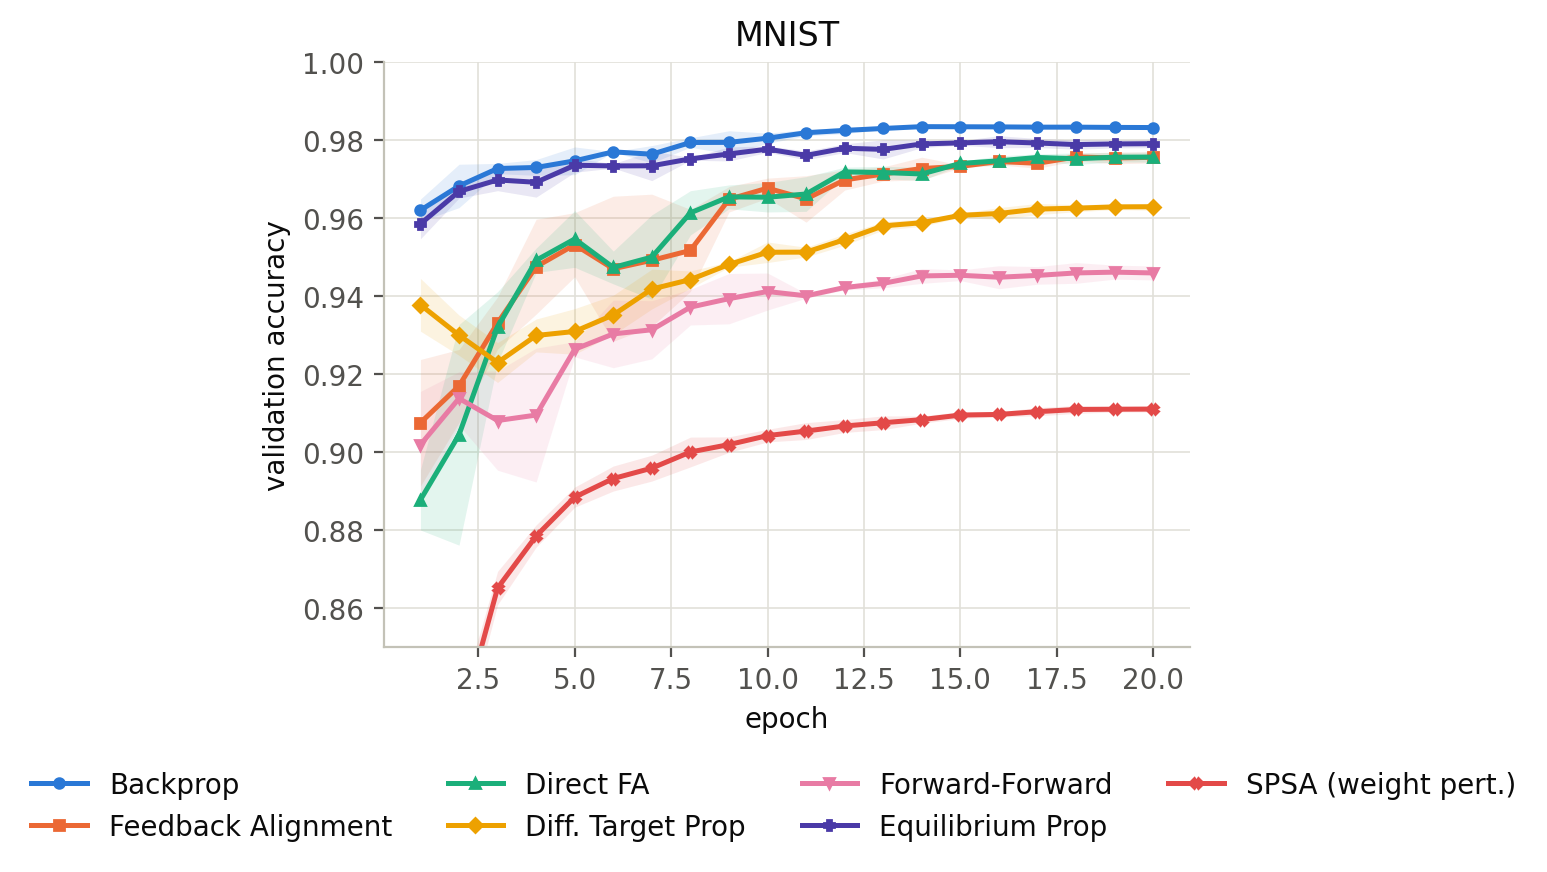
\includegraphics[width=\linewidth]{fig_learning_curves.png}\caption{Validation accuracy per epoch (mean $\pm$ std over seeds).}\end{figure}
BP reaches $98.47\pm0.06\%$ test accuracy. EqProp is the closest alternative ($97.91\pm0.14\%$), followed by FA ($97.53\%$) and DFA ($97.50\%$), DTP ($95.96\%$), FF ($94.35\%$) and SPSA ($90.76\%$). All methods except FF and SPSA fit the training set almost perfectly ($\ge97.5\%$ train accuracy), so the differences are mainly differences in how well the update direction optimises. The train--test gap is $1.5$ points for BP, $1.6$ for DTP, $1.9$ for EqProp, $2.0$ for FA and $2.2$ for DFA, i.e.\ the alternatives with more aligned-but-biased updates do not generalise better than BP here. FF (which uses $3\times500$ hidden units, i.e.\ 3.8$\times$ the parameters) under-fits (train $94.7\%$, gap $0.36$ points), consistent with public re-implementations, and is below the numbers of the original paper, which uses larger networks and more training. SPSA is also under-fitted and, importantly, was the only method whose stability required an extra device (update-norm clipping): with $k=16$ its update has, in expectation, a norm $\approx\sqrt{d/k}\approx120$ times that of the true gradient. \todo{Fashion-MNIST: repeat this paragraph.}

\subsection{Quality of the update direction}
\begin{figure}[h]\centering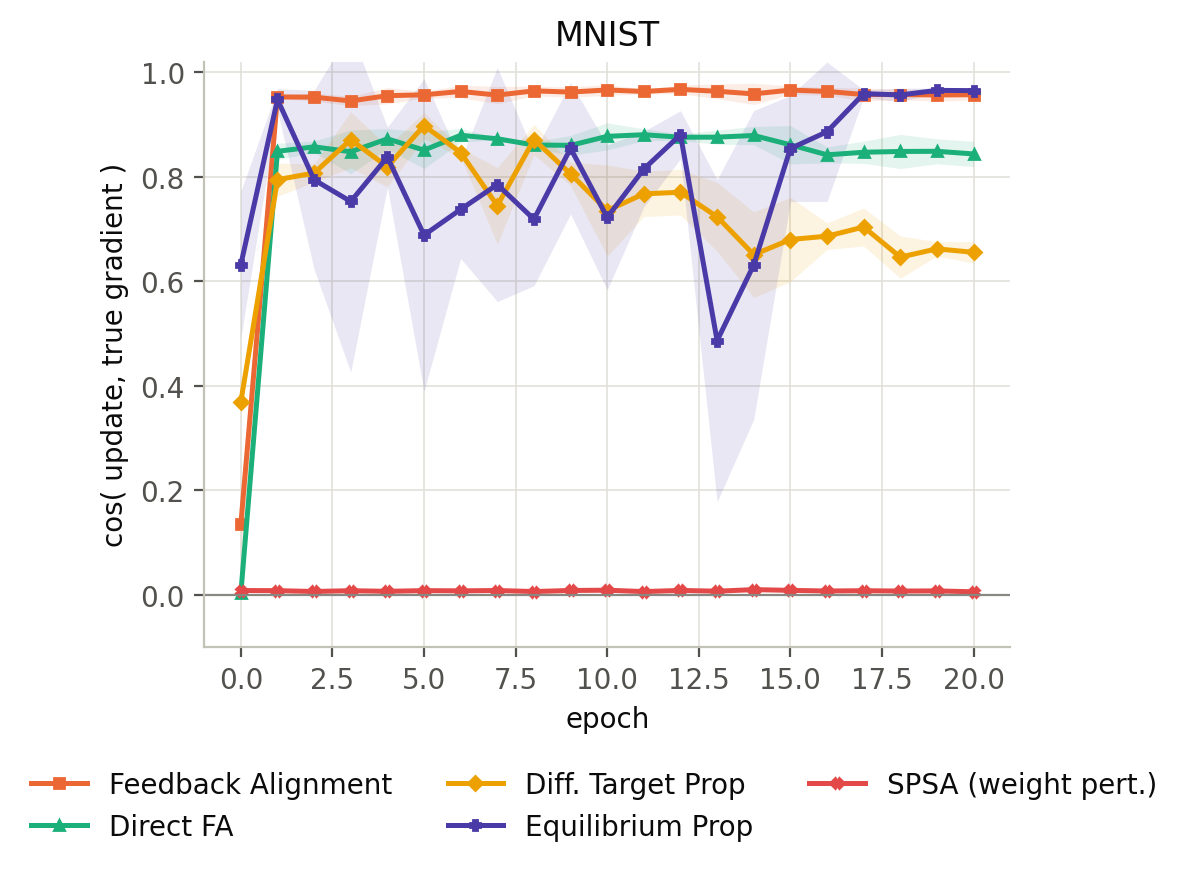
\includegraphics[width=.9\linewidth]{fig_gradient_alignment.png}\caption{Cosine between each method's update and the true gradient during training.}\end{figure}
\begin{figure}[h]\centering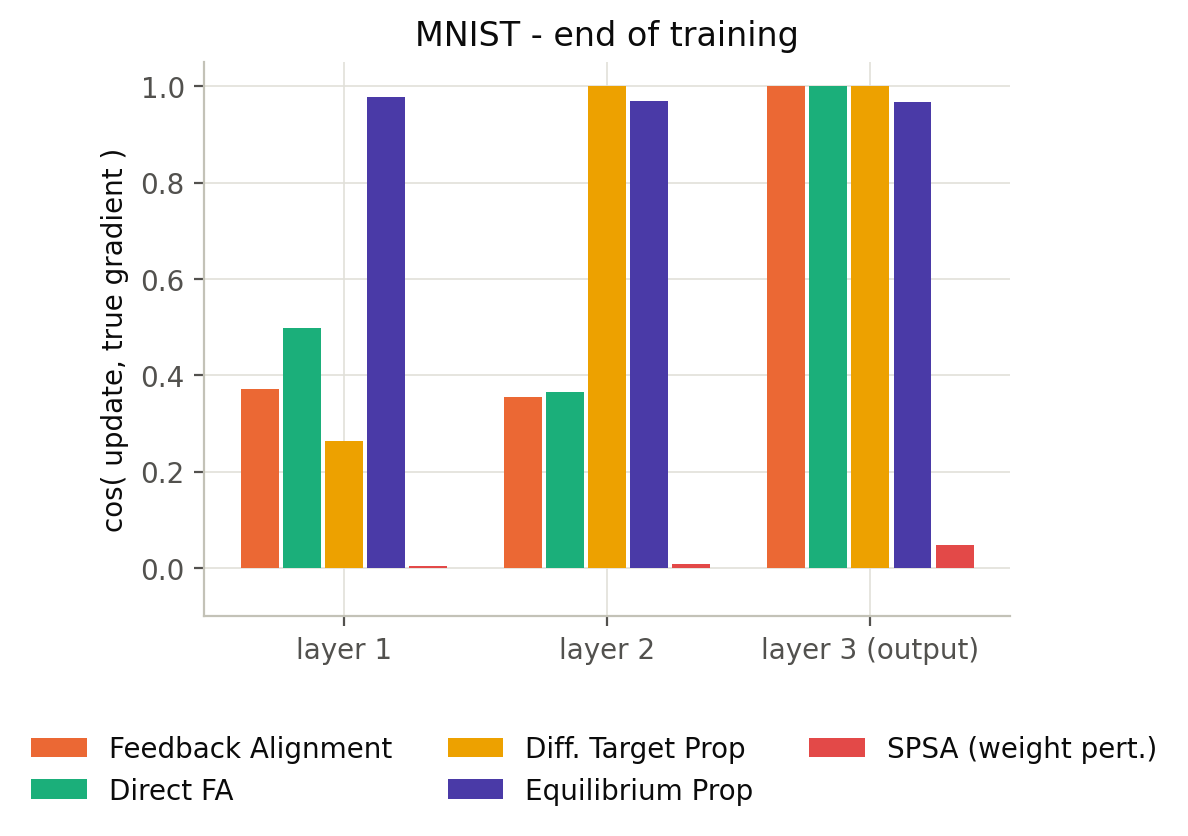
\includegraphics[width=.9\linewidth]{fig_alignment_per_layer.png}\caption{Per-layer alignment at the end of training (layer 3 is the output layer, whose update is exact for FA/DFA).}\label{fig:layers}\end{figure}
Starting from an alignment of $0.14$ at initialisation, FA reaches $0.95$ within the first epoch and stays at $0.96$, in line with the ``align, then memorise'' picture \cite{refinetti2021}. The global number is misleading, however: the output-layer update of FA and DFA is exact, and it dominates the gradient norm. Per layer (Fig.~\ref{fig:layers}) the hidden-layer cosines at the end of training are only $0.37/0.36$ (FA) and $0.50/0.37$ (DFA). DTP's top hidden layer receives a true gradient step by construction (cosine $1.0$) while its first hidden layer aligns only at $0.26$. EqProp's update is the only one aligned across all layers ($0.97$--$0.98$), but this alignment fluctuates during training between $0.5$ and $0.97$: with the tuned $\beta=0.25$ the estimator is biased (Fig.~\ref{fig:eq-spsa}, left: cosine $0.63$ at $\beta=0.25$, $0.91$ at $0.1$, $0.998$ at $0.01$), yet the method still trains well, so \emph{exactness of the gradient is not necessary for good accuracy}. SPSA's alignment is $0.006$ ($0.05$ for the 1290-parameter output layer), matching $\sqrt{k/(d+k)}$ (Fig.~\ref{fig:eq-spsa}, right).

\subsection{EqProp converges to the gradient; SPSA needs many directions}
\begin{figure}[h]\centering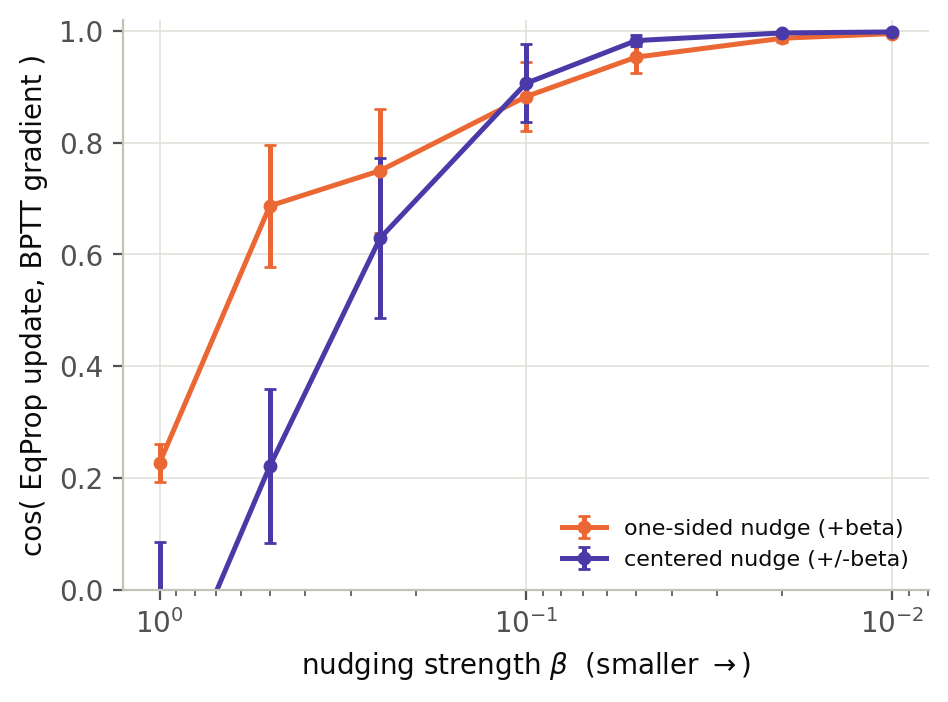
\includegraphics[width=.48\linewidth]{fig_eqprop_beta.png}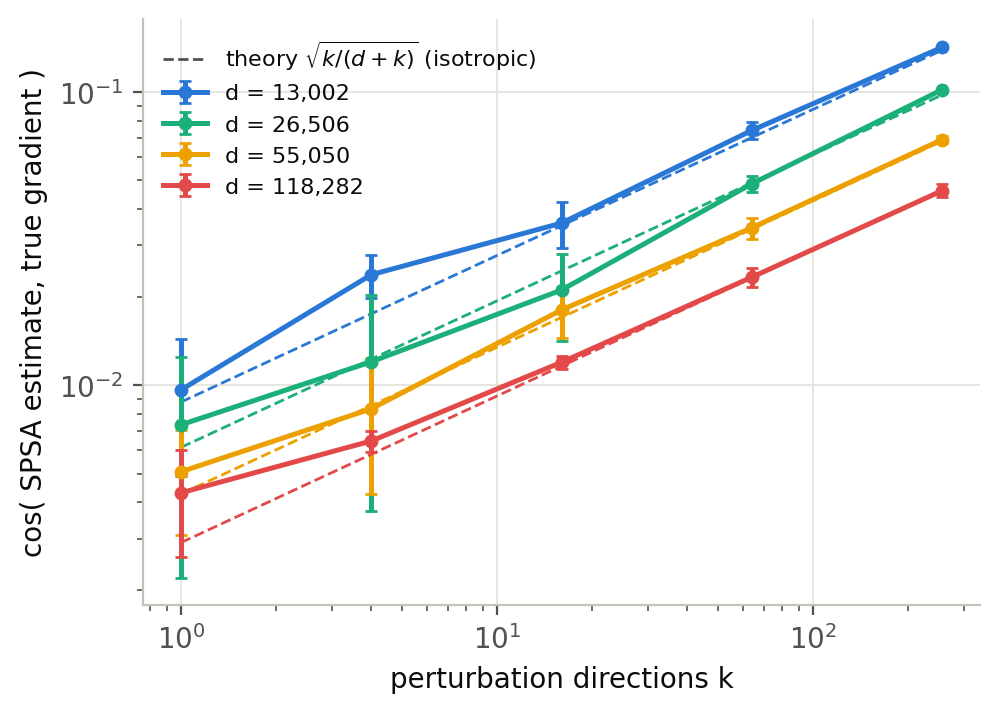
\includegraphics[width=.48\linewidth]{fig_spsa_variance.png}\caption{Left: EqProp update vs.\ BPTT gradient as $\beta\to0$ (theory: exact in the limit). Right: SPSA alignment vs.\ number of directions $k$ for several parameter counts $d$; dashed: $\sqrt{k/(d+k)}$.}\label{fig:eq-spsa}\end{figure}

\subsection{Depth and data efficiency}
With 2/3/4/6 hidden layers BP stays at $98.3$--$98.4\%$ (2--4 layers) and $98.2\%$ (6). FA drops $97.1\to95.2\to93.7\to89.2\%$, DFA $97.2\to95.7\to94.1\to92.3\%$, DTP $95.4\to91.3\to82.3\to26.0\%$. EqProp is competitive up to 4 layers ($98.0, 97.7, 97.3\%$) but with fixed hyper-parameters (relaxation length scaled with depth) one of two seeds fails to train at 6 layers (mean $58.8\%$), we did not diagnose the cause (a natural suspect is loss of stability of the relaxation dynamics in deeper coupled networks; checking the spectral radius of the Jacobian is left to future work). Data efficiency (fixed number of gradient steps): with 1\,000 examples the spread between best and worst method is $4.4$ points ($89.7\%$ BP vs.\ $85.3\%$ FF); with 50\,000 it is $9.7$ points; SPSA barely improves with more data ($85.9\to88.7\%$), since it is optimisation-limited.
\begin{figure}[h]\centering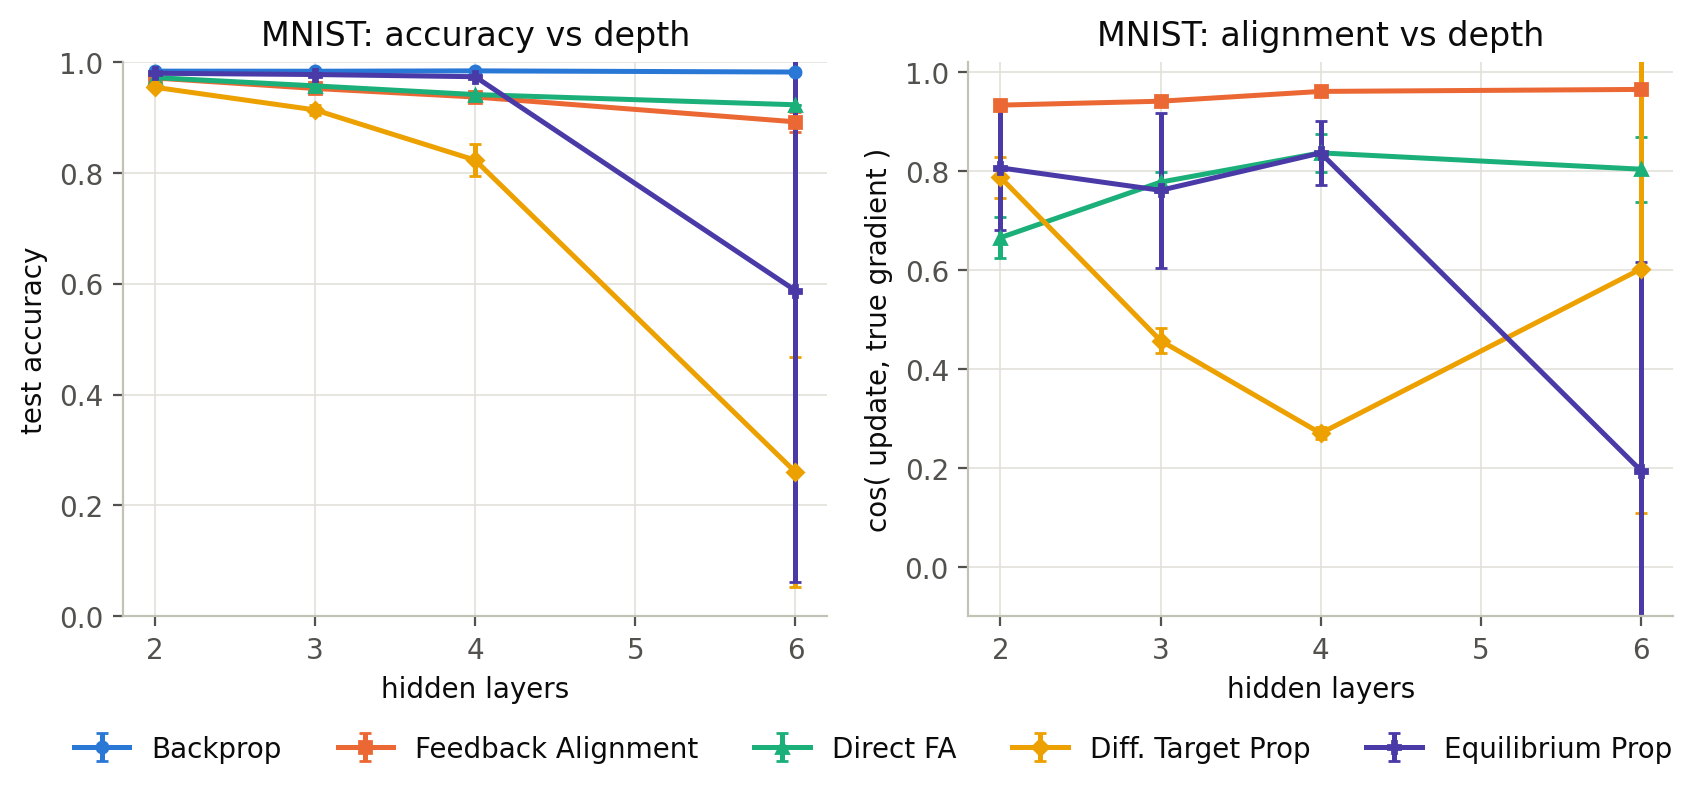
\includegraphics[width=\linewidth]{fig_depth.png}\caption{Accuracy and alignment vs.\ number of hidden layers.}\end{figure}
\begin{figure}[h]\centering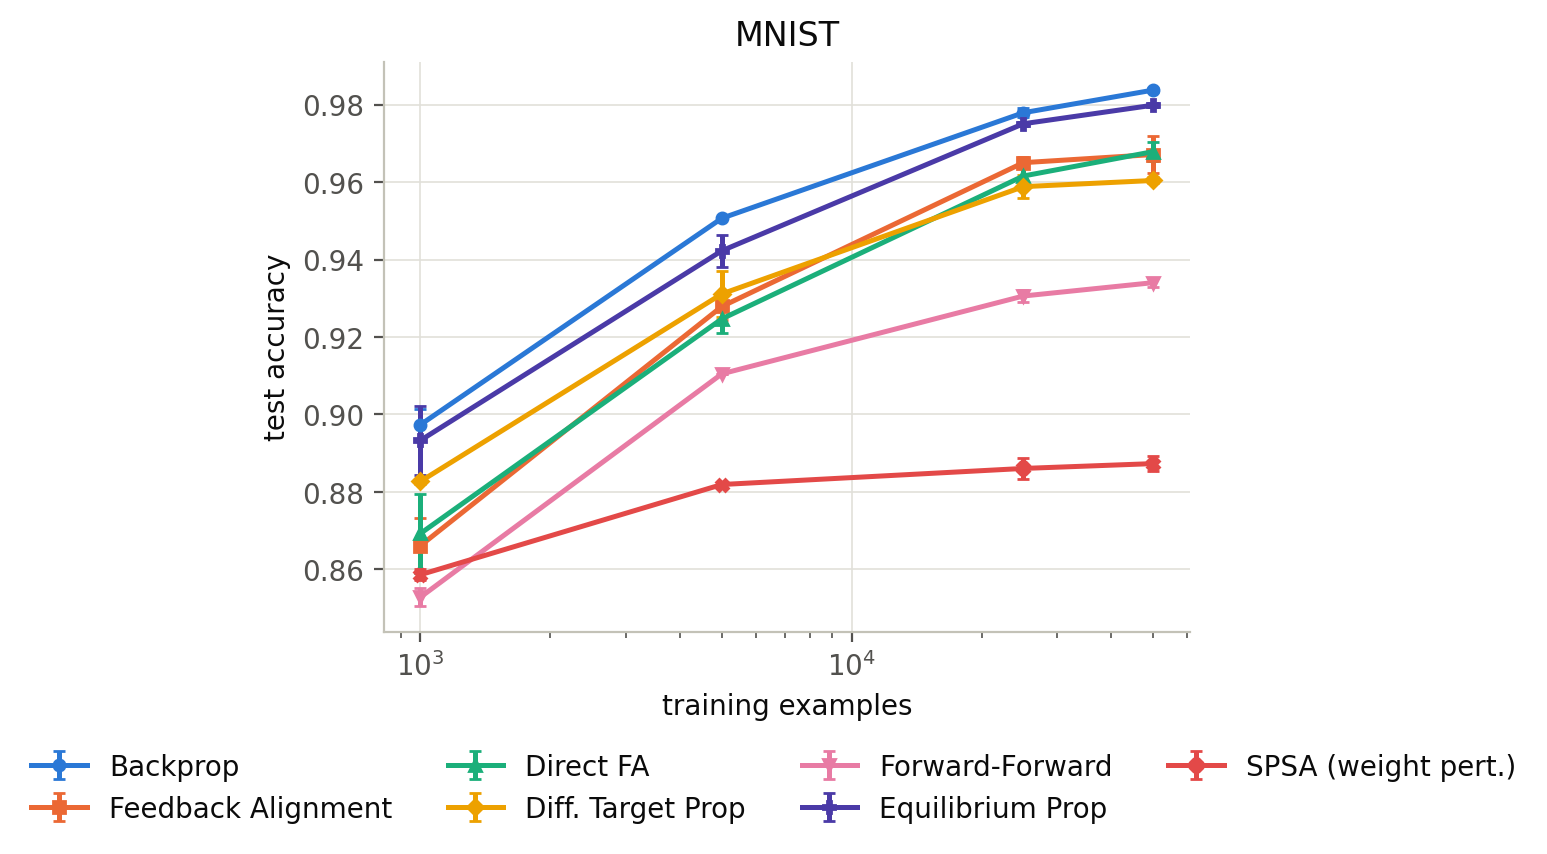
\includegraphics[width=.9\linewidth]{fig_data_efficiency.png}\caption{Test accuracy vs.\ training-set size at a fixed number of gradient steps.}\end{figure}

\subsection{Computational cost}
\begin{figure}[h]\centering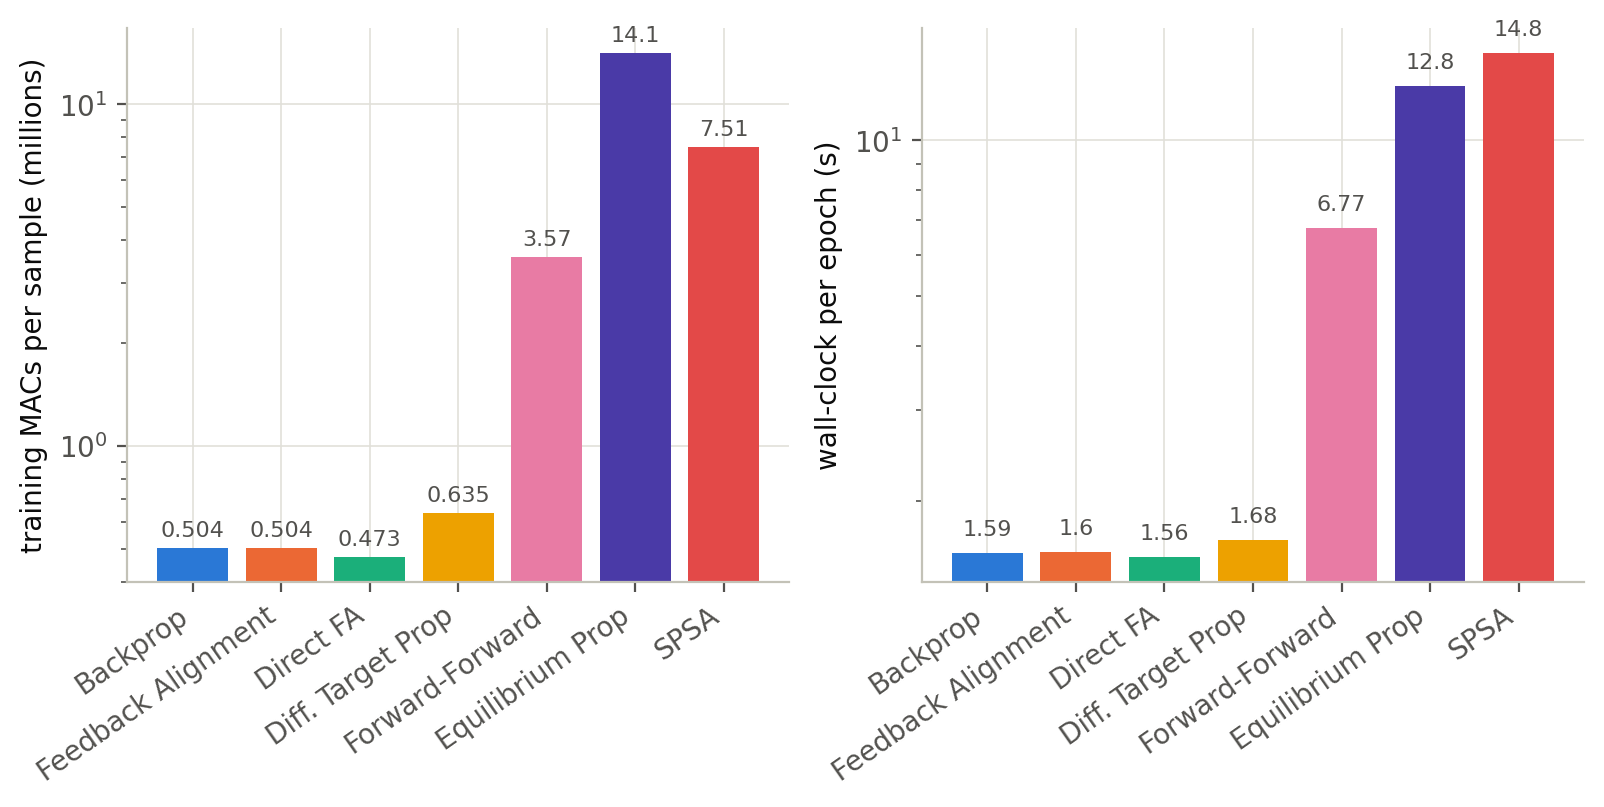
\includegraphics[width=.8\linewidth]{fig_compute_cost.png}\caption{Measured training cost per sample.}\end{figure}
\begin{figure}[h]\centering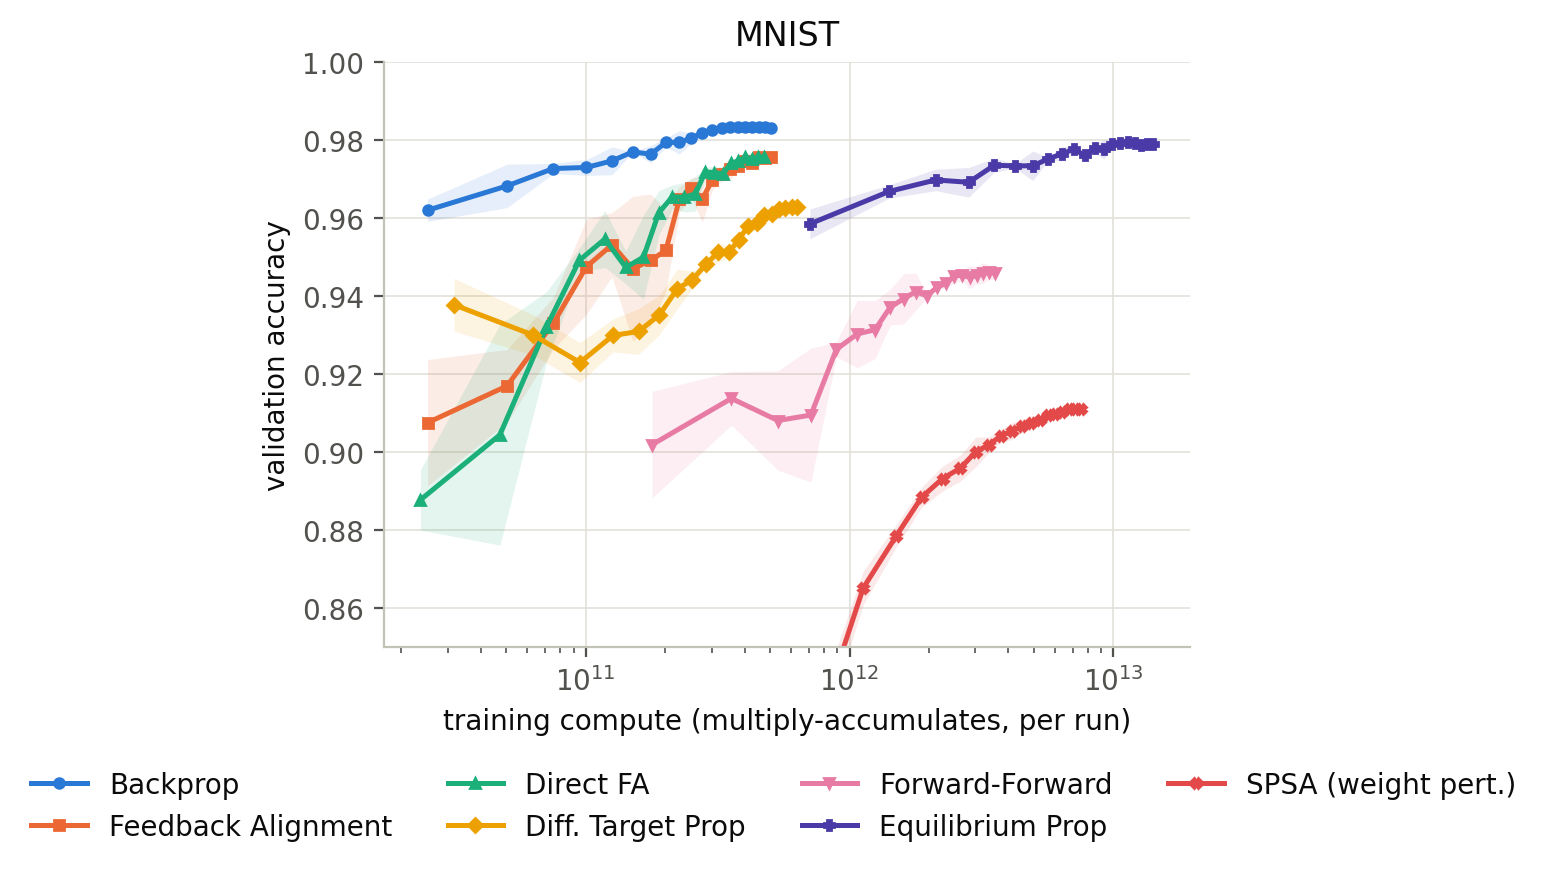
\includegraphics[width=.9\linewidth]{fig_acc_vs_compute.png}\caption{Validation accuracy against cumulative multiply-accumulates.}\end{figure}

\section{Discussion}
\paragraph{Provably vs.\ empirically convergent.} EqProp is the only method with a convergence guarantee to the true gradient (as $\beta\to0$), and we confirm it numerically. FA has none, but empirically aligns fast in shallow nets and degrades with depth. In practice both regimes coexist: the ``provable'' method was used at a large $\beta$ where it is biased, and still worked best of the alternatives.
\paragraph{Cost.} Locality is not free. EqProp needs a relaxation (here $30+2\times10$ steps) per update, $28\times$ the MACs of BP; SPSA needs $2k$ forward passes ($15\times$); FF processes positive and negative data and $10$ label hypotheses at inference. FA/DFA cost the same as BP on a GPU; their advantage is hardware-side (no weight transport), not FLOPs.
\paragraph{Limitations.} A single small MLP, two datasets, three seeds (two for depth/data), one hyper-parameter budget; no convolutional or large-scale experiments, where FA/DTP/FF are known to be much weaker \cite{bartunov2018,xiao2018,launay2020}. Hyper-parameters were tuned on MNIST and (unless re-tuned) reused for Fashion-MNIST. \todo{Hebbian/STDP learning is not covered.}

\section{Conclusion}
In a controlled small-scale comparison, no alternative matches BP at equal cost; the closest (EqProp) pays with an order of magnitude more computation, and the cheap ones (FA, DFA) lose accuracy that grows with depth because their hidden-layer updates are only weakly aligned with the gradient. Methods that dispense with a global error path entirely (FF, SPSA) trail by 4--8 points on MNIST. \todo{Fashion-MNIST sentence.}

\bibliographystyle{plain}
\bibliography{refs}
\end{document}
